\section{Implementation Details}\label{sec:Implementation}

The chaincode is written in Golang and provides all contracts needed to proceed traceability in the application. All contracts for use in chaincode must implement the interface \textit{contractapi.ContractInterface}. 

The first step is to create a JSON config file providing all information about these three items. A configuration file includes \textit{assetId}, a list of actors and a list of ordered steps. The chaincode processes this file through  \textit{initLedger} and \textit{createNewAsset} functions. Here follows a template for config file:  

\begin{minted}{json}
{
   "AssetId":"assetID",
   "AssetName":"assetName",
   "AssetDescription":"assetDescription",
   "Actors":[
      {
         "actorType":"type",
         "aditionalInfo":[
            {
               "key":"value"
            }
         ]
      }
   ],
   "Steps":[
      {
         "StepId":"stepID",
         "StepName":"stepName",
         "StepOrder":1,
         "ActorType":"actorType",
         "aditionalInfo":[
            {
               "key":"value"
            }
         ]
      }
   ]
}
\end{minted}

Front-end WebApp enables a user to define settings through a Configuration Page, adding these to the configuration file, as shown in Figure~\ref{fig:create_asset_4}.

Assets, asset items, steps and actors are described as \textit{structs}, as follows:

\begin{minted}{go}
type Actor struct {
  ActorId    string  `json:"actorId"`
  ActorType  string  `json:"actorType"`
  ActorName  string  `json:"actorName"`
  Deleted    bool    `json:"deleted"`
  AditionalInfo map[string]string `json:"  aditionalInfo"`
}

type Step struct {
  StepId     string  `json:"stepId"`
  StepName   string  `json:"stepName"`
  StepOrder  uint    `json:"stepOrder"`
  ActorType  string  `json:"actorType"`
  Deleted    bool    `json:"deleted"`
  AditionalInfo map[string]string `json:"  aditionalInfo"`
}

type AssetItem struct {
  AssetItemId   string    `json:"assetItemId"`
  OwnerId       string    `json:"ownerId"`
  StepID        string    `json:"stepID"`
  ParentID      string    `json:"parentID"`
  Children      []string  `json:"children"`;
  ProcessDate   string    `json:"processDate"`
  DeliveryDate  string    `json:"deliveryDate"`
  OrderPrice    string    `json:"orderPrice"`
  ShippingPrice string    `json:"shippingPrice"`
  Status        string    `json:"status"`
  Quantity      string    `json:"quantity"`
  Deleted       bool      `json:"deleted"`
  AditionalInfo map[string]string `json:"  aditionalInfo"`
}

type Asset struct {
  AssetId      string       `json:"assetId"`
  AssetName    string       `json:"assetName"`
  Description  string       `json:"description"`
  AssetItems   []AssetItem  `json:"assetItems"`
  Actors       []Actor      `json:"actors"`
  Steps        []Step       `json:"steps"`
  Deleted      bool         `json:"deleted"`
  AditionalInfo map[string]string `json:"aditionalInfo"`
}
\end{minted}

There are create methods for each one,  responsible for creating an instance of these \textit{structs} and save the state into the Blockchain. Query methods are responsible for interact with the information of any item in the Blockchain.


The chaincode \textit{main} function invokes the \textit{initLedger} function, reads the configuration files and raises the platform enabling users to interact with the Blockchain via exposing its API, as follows: 

\begin{minted}{go}
func main() {
  chaincode, err := contractapi.NewChaincode(new(SmartContract))
  if err != nil {
    fmt.Printf("Error create chaincode: %s", err.Error())
    return
  }
  if err := chaincode.Start(); err != nil {
    fmt.Printf("Error starting chaincode: %s", err.Error())
  }
}
\end{minted}

When creating an asset item, an \textit{AssetItemId} is generated. Each entity in the chain will have its unique entity ID and timestamp when it starts processing the transaction. By querying \textit{AssetItemId}, the user can easily track the current transaction information and status. Finally, completed all steps, the Blockchain will update \textit{deliverDate} and mark the status as completed once the last actor (generally the consumer) has received the order. Here follows \textit{CreateAsset} function:

\begin{minted}{go}
func (s *SmartContract) CreateAsset(
  ctx contractapi.TransactionContextInterface, assetId string,
  assetName string, description string, assetItems []AssetItem, 
  actors []Actor, steps []Step, aditionalInfo map[string]string) error {
  
  if err != nil {
    return fmt.Errorf(
      "Failed to read the data from world state: %s", err
    )
  }

  if assetJSON != nil {
    return fmt.Errorf("The asset %s already exists", assetID)
  }
  
  asset := Asset {
    AssetId:       assetId,
    AssetName:     assetName,
    Description:   description,
    AssetItems:    assetItems,
    Actors:        actors,
    Steps:         steps,
    Deleted:       false,
    aditionalInfo: aditionalInfo,
  }
  assetAsBytes, _ := json.Marshal(asset)
  if err != nil {
    return err
  }
  return ctx.GetStub().PutState("ASSET_"+assetId,assetAsBytes)
}
\end{minted}

\textit{MoveAssetItem} is the method called to update an asset item when it is moved from a step to another. It updates the \textit{CurrentOwnerId}, the \textit{ProcessDate}, information about prices and many other details of the transactions by the key/value map \textit{  aditionalInfo}. Here follows this fuction:

\begin{minted}{go}
func (s *SmartContract) MoveAssetItem(
  ctx contractapi.TransactionContextInterface, 
  assetItemID string, newAssetItemID string, stepID string, 
  newOwnerID string, orderPrice string, shippingPrice string, 
  status string, quantity string, 
  aditionalInfo map[string]string ) error {
  
  assetItemJSON, err := s.QueryAssetItem(ctx, assetItemID)
  if err != nil {
    return err
  }
  if assetItemJSON == nil {
    return fmt.Errorf("The assetItem %s does not exists", assetItemID)
  }

  newAssetItem := AssetItem{
    AssetItemID:      newAssetItemID,
    OwnerID:          newOwnerID,
    StepID:           stepID,
    ParentID:         assetItemID,
    Children:         []string{},
    ProcessDate:      time.Now().Format("2006-01-02 15:04:05"),
    OrderPrice:       orderPrice,
    ShippingPrice:    shippingPrice,
    Status:           status,
    Quantity:         quantity,
    Deleted:          false,
    AditionalInfoMap: aditionalInfo,
  }

  assetItemAsBytes, err := json.Marshal(newAssetItem)
  if err != nil {
    return err
  }

  return ctx.GetStub().PutState(
    "ASSET_ITEM_"+newAssetItemID, assetItemAsBytes
  )
}
\end{minted}

\textit{TrackAssetItem} is the method responsible for track an asset item. It returns the children tree of the given element and its ancestors from the beginning of the Supply chain. This method uses the function getChildenTree to get the current item's children nodes: 

\begin{minted}{go}
func (s *AssetTransferSmartContract) TrackAssetItem(
  ctx contractapi.TransactionContextInterface, 
  assetItemID string) ([]*AssetItem, error) {
  
  assetItem, err := s.QueryAssetItem(ctx, assetItemID)
  log.Print("tracking info from assetItem id: ", assetItem.AssetItemID)
  if err != nil {
    return nil, fmt.Errorf(
      "Failed to read from world state. %s", err.Error()
    )
  }

  if assetItem == nil {
    return nil, fmt.Errorf("%s does not exist", assetItemID)
  }

  trackedItems := make([]*AssetItem, 0)

  //first add the children to tracked items
  children, err := s.getChildenTree(ctx, assetItem)
  if err != nil {
    return nil, fmt.Errorf(
      "Failed to read from world state. %s", err.Error()
    )
  }

  for _, child := range children {
    fmt.Println(child)
    trackedItems = append(trackedItems, child)
  }

  //then, add the current item to tracked items
  trackedItems = append(trackedItems, assetItem)

  //finally, add the ancestor of current item to tracked items
  for {
    currentParentId, err := strconv.Atoi(assetItem.ParentID)
    if (currentParentId <= 0) {
      break
    }
    parentAssetItem, err := s.QueryAssetItem(ctx, assetItem.ParentID)
    if err != nil {
      return nil, fmt.Errorf(
        "Failed to read from world state. %s", err.Error()
      )
    }
    newParentId, err := strconv.Atoi(parentAssetItem.ParentID)
    log.Print("newParentId: ", newParentId)
    trackedItems = append(trackedItems, parentAssetItem)
    assetItem = parentAssetItem
  }
  return trackedItems, nil
}

func (s *AssetTransferSmartContract) getChildenTree(
  ctx contractapi.TransactionContextInterface, 
  assetItem *AssetItem) ([]*AssetItem, error) {
  
  tree := make([]*AssetItem, 0)
  log.Print("len(assetItem.Children): ", len(assetItem.Children))
  if len(assetItem.Children) == 0 {
    tree = append(tree, assetItem)
  } else {
    for _, childId := range assetItem.Children {
      childAssetItem, err := s.QueryAssetItem(ctx, childId)
      if err != nil {
        return nil, fmt.Errorf(
          "Failed to read from world state. %s", err.Error()
        )
      }
      if childAssetItem == nil {
        return nil, fmt.Errorf("%s does not exist", childId)
      }

      childrenTree, err := s.getChildenTree(ctx, childAssetItem)
      for _, child := range childrenTree {
        tree = append(tree, child)
      }
    }
    tree = append(tree, assetItem)
  }
  return tree, nil
}
\end{minted}


Figure~\ref{fig:sequenceDiagram} shows the interaction flow from users with Árion platform. Initially, an admin persona creates and configure the SCM, adding information about the steps and the users. After that, the admin can activate this SCM, and from that point, the actors can interact with the SCM to provide information about an asset item and also move this asset item through the supply chain. From that point too, any user can track an asset item to get information about the required good.

%htbp
\begin{figure}[ht]
\begin{center}
  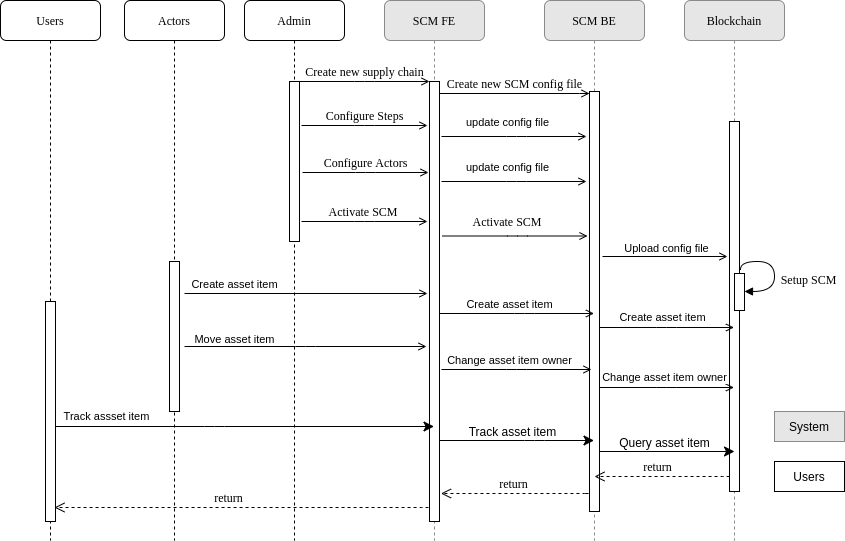
\includegraphics[scale=0.5]{images/SequenceDiagram.png}
\caption{SCM User flow}
\label{fig:sequenceDiagram}
\end{center}
\end{figure}


The backend gateway exposes all the endpoints shown in table \ref{table:endpoints}. These endpoints are integrated with the frontend and can be used in the future work to integrate with a mobile app or an external application.


\begin{table}[htb]
\centering
\caption{Backend endpoints}
\label{table:endpoints}
    \begin{center}
    \begin{tabular}{|l|p{4.5cm}|p{7.664cm}|}
        \hline 
        \thead{Verb} & \thead{URI} & \thead{Description}\\
        \hline 
        \cellcolor{cyan}\textbf{Actors}  & \cellcolor{cyan}\textbf{} & \cellcolor{cyan}\textbf{} \\
        \hline 
        POST & /actors & creates a new actor\\
        \hline 
        GET & /actors & retrieves the actors' list\\
        \hline 
        PUT & /actors/:id & updates an existing actor\\
        \hline 
        GET & /actors/:id & retrieves an existing actor\\
        \hline 
        DELETE & /actors/:id & removes an existing actor\\
        \hline 
        \cellcolor{cyan}\textbf{Steps}  & \cellcolor{cyan}\textbf{} & \cellcolor{cyan}\textbf{} \\
        \hline 
        POST & /steps & creates a new step\\
        \hline 
        GET & /steps & retrieves the steps' list\\
        \hline 
        PUT & /steps/:id & updates an existing step\\
        \hline 
        GET & /steps/:id & retrieves an existing step\\
        \hline 
        DELETE & /steps/:id & removes an existing step\\
        \hline 
        \cellcolor{cyan}\textbf{Asset Items}  & \cellcolor{cyan}\textbf{} & \cellcolor{cyan}\textbf{} \\
        \hline 
        POST & /asset-items & creates a new asset item\\
        \hline 
        GET & /asset-items & retrieves the asset items' list\\
        \hline 
        PUT & /asset-items/:id & updates an existing asset item\\
        \hline 
        GET & /asset-items/:id & retrieves an existing asset item\\
        \hline 
        DELETE & /asset-items/:id & removes an existing asset item\\
        \hline 
        POST & /asset-items/:id & moves an asset item through the SCM\\
        \hline 
        GET & /asset-items/track/:id & tracks an asset item through the SCM\\
        \hline
        \cellcolor{cyan}\textbf{Assets}  & \cellcolor{cyan}\textbf{} & \cellcolor{cyan}\textbf{} \\
        \hline 
        POST & /assets & creates a new asset\\
        \hline 
        GET & /assets & retrieves the assets' list\\
        \hline 
        PUT & /assets/:id & updates an existing asset\\
        \hline 
        GET & /assets/:id & retrieves an existing asset\\
        \hline 
        DELETE & /assets/:id & removes an existing asset\\
        \hline 
    \end{tabular}
    \end{center}
\end{table}
